\chapter{Analyse des opportunités des technologies libres dans le
domaine de l'édition vidéo et prévisions}

\minitoc \newpage

\paragraph{}

Maintenant que les besoins et que les solutions existantes ont été
analysées on rendra compte de la situation actuelle des technologies
libres et de leurs communautés. Il est aussi important de chercher
les raisons qui expliquent que ces logiciels ne sont pas plus utilisés
par les professionnels. Puis, nous essayerons d'envisager les solutions
possibles qui permettraient de remédier à cette situation.

\paragraph{}

Dans cette partie, nous analyserons la différence entre les manières
d'envisager la création de logiciel et nous verrons quels sont les
avantages et inconvénients de ces fonctionnements. Par la suite nous
nous concentrerons sur les frameworks existants pour faire une analyse
technique de ces technologies. Puis, nous analyserons les communautés
qui portent ces différents projets afin de déterminer les points forts
et les points faibles de chacun des projets.  Pour finir, nous tirerons
les conclusions de cette analyse afin de trouver des solutions aux défis
qu'est la création d'un logiciel libre de montage vidéo.

\newpage

\section {Etat actuel de l'offre de logiciel libre}

Le schéma suivant permet de résumer facilement la situation:

\begin{figure} [h]
  \begin{center}
    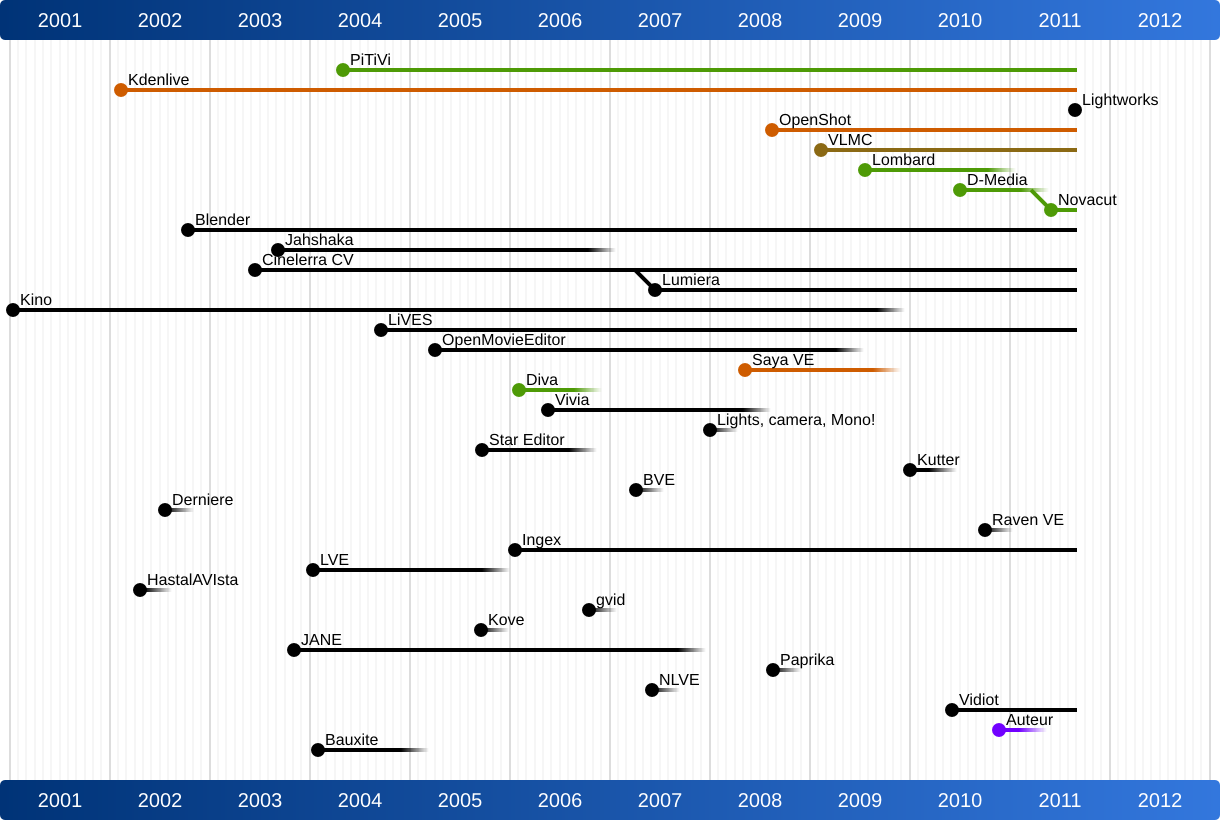
\includegraphics[width=0.9\textwidth]{images/open-source-video-editor-timeline}
  \end{center} \caption{Open source video editors timeline (Auteur:
  Jean-François Fortin Tam, PiTiVi designer)} \label{Yes}
\end{figure}

\paragraph{ }

On constate donc que de nombreux projets de logiciel libre de montage
vidéo on vu le jours ces 10 dernières années et dont les objectifs
sont différents.  On peut distinguer deux types de public visés par
ces projets:

\begin {itemize}

  \item {Les amateurs}

  \item {Les professionnels ou semi professionnels}
\end {itemize}

\paragraph {Les amateurs de montages vidéo}

\subparagraph{}

Plusieurs projets libres permettent ou visent à répondre aux besoins
des amateurs, mais à l'heure actuelle ils ne sont que partiellement
adaptés à ces besoins. Parmi les logiciels dont l'objectif est de
permettre de créer des montages simples on distingue:

\begin {itemize}

  \item {openshot: Logiciel présentant  de nombreuses fonctionnalités,
  mais dont la
    qualité d'implémentation présente des faiblesses.}

  \item {kino: Logiciel avec un nombre de fonctionnalités limité
  permettant de faire des petit montages avec efficacité.}

  \item {Vidiot qui vise la production de vidéo amateur simple}

\end {itemize}

\paragraph {}

Mais il existe des logiciels ayant pour objectif de répondre aux besoins
plus avancés en particulier à ceux des professionnels (précédemment
présenté dans le cadre de la définition des plus grands acteurs du
marché) qui peuvent être utilisés dans le cadre de montage amateur.
Leur utilisation (et c'est plus particulièrement le cas du logiciel
Cinelerra) demeure complexe.

\paragraph{}

Un nouveau projet a aussi récemment vu le jour, dont la finalité est
assez différente des logiciels actuellement présents. Il s'agit de
Novacut, qui permet aux créateurs de films et séries web de faire le
montage de manière collaborative à travers d'Internet en partageant
les ressources (footage).

\paragraph{}

% Human readable version:

% Le fait que Cinelerra ne soit packagé dans aucune distribution

% Linux montre que même ce logiciel est le seul à avoir réussi à

% prendre une part de marché dans le milieu de l'édition

% professionnelle, celui-ci n'a pas réussi à rassembler les

% développeurs et utilisateurs standard de logiciel libre.

Le fait que Cinelerra ne soit packagé \footnote{Packagé: fait
que qu'un paquet, une archive (fichier compressé) comprenant les
fichiers informatiques, les informations et procédures nécessaires
à l'installation d'un logiciel sur un système d'exploitation au sein
d'un agrégat logiciel, en s'assurant de la cohérence fonctionnelle
du système ainsi modifié ait été créé. Source: Wikipedia} dans
aucune distribution Linux \footnote {Une distribution Linux, appelée
aussi distribution GNU/Linux pour faire référence aux logiciels du
projet GNU, est un ensemble cohérent de logiciels, la plupart étant
logiciels libres, assemblés autour du noyau Linux. Source: Wikipedia}
montre que même ce logiciel est le seul à avoir réussi à prendre
une part de marché dans le milieu de l'édition professionnelle,
il n'a toutefois pas su susciter l'enthousiasme des développeurs et
utilisateurs typiques de la communauté du logiciel celui-ci n'a pas
réussi à rassembler les développeurs et utilisateurs standard de
logiciel libre. Nous verrons les raison techniques qui expliquent ce fait.

\paragraph{}

En définitive aucun projet n'a encore réussi à s'imposer et ainsi
regrouper les développeurs au sein de projets majeurs. Dans d'autre
domaines, cela a été le cas, par exemple dans le domaine des lecteurs
vidéo, Vlc a su surpasser ses concurrents, et ainsi supplanter le
marché des lecteurs vidéo, qu'il soit libre ou non. Dans le domaine
des environnements de Bureau graphique, KDE et Gnome sont arrivés à un
stade où leur supériorité technique, et en terme de fonctionnalités,
fait d'eux des plateformes de référence.

\paragraph{}

Il est donc intéressant de se demander quelles technologies et quels
logiciel(s), pourraient se voir attribuer cette place dans le monde
de l'édition vidéo libre. Nous allons donc analyser les logiciels et
les technologies libres les plus avancés, (précédemment mentionnés
dans le cadre de l'analyse de marché: Cinelerra, Kdenlive et PiTiVi).
Nous verrons ainsi s'ils ont le potentiel de pouvoir un jour rivaliser
avec les logiciels propriétaires sur le marché très fermé du montage
vidéo professionnel.

\paragraph{}

NB: Il aurait été intéressant d'analyser le logiciel lightworks,
en voie de libération, mais à l'heure actuelle, aucun code n'a été
libéré, et par conséquent, celui-ci ne peut pas faire partie de
cette analyse.

\newpage

\section{Technologies}

\paragraph{}

Pour faire une analyse technique des produits permettant de faire
de l'édition vidéo, il est nécessaire d'analyser le ``core'' des
logiciels, c'est à dire la partie du logiciel où les opérations
d'édition sont effectivement réalisées. Dans ces domaines, il existe
deux façon de procéder:

\begin{itemize} \setlength{\itemsep}{2mm}

  \item{Création d'un logiciel monolithique\index{monolithique}}

  \item{Création d'un framework \glossary {name={framework},
   description={Un framework est un ensemble d'outils et de composants
   logiciels organisés conformément à un plan d'architecture et des
   designs patterns (un patron de conception, motif de conception ou
   modèle de conception est un concept de génie logiciel destiné à
   résoudre les problèmes récurrents suivant le paradigme objet.)}}
   \index{framework}}

\end{itemize}

\subsection {Technologies monolithiques\index{monolithique} VS
technologies modulaires, frameworks}


\subsubsection{Logiciels monolithiques \index{monolithique}}

\paragraph{}

Le conception monolithique \index{monolithique} dans le cadre des
logiciels d'édition vidéo, consiste à développer au sein d'un même
entité de code:

\begin{itemize} \setlength{\itemsep}{2mm}

  \item {la partie graphique et la partie de calculs
    permettant la gestion de tout ce que l'édition non linéaire
    implique}

  \item {L'interface utilisateur.}

\end {itemize}

\paragraph{}

Par le terme logiciel monolithique\index{monolithique}, il faut réaliser
que le logiciel peut utiliser des librairies externes, mais le core
de ce même logiciel, et la logique d'édition linéaire à proprement
parler sont directement élaborés à l'intérieur du logiciel et non
par une librairie ou framework \index{framework} externe. Cela a pour
principal avantage de présenter une conception simplifiée pour les
raisons suivantes:

\paragraph{}

Les logiciels professionnels (commerciaux) utilisent très probablement
tous ce mode de fonctionnement (même si vraisemblablement,
en interne il ont un core qui ressemble fortement à un framework
\index{framework}).Dans le monde des logiciels libres,les développeurs
de Cinelerra ont décidé d'utiliser ce mode de fonctionnement.

On peut voir plusieurs conséquences immédiates de ce mode de
développement:

\begin{itemize} \setlength{\itemsep}{2mm}

  \item {Les développeurs n'ont pas la nécessité de penser
    en terme d'interface publique de programmation (API\index{API}), et
    n'ont pas à garantir la stabilité de celle-ci: le risque réside
    dans le fait que la qualité de l'architecture ne soit pas optimale
    car la création d'API\index{API} oblige les développeurs/architectes
    à réellement analyser les besoins de manière plus large dès
    le début de la conception. Dans le cas où l'on ne crée pas
    d'interface publique de programmation vouée à être réutilisée,
    le risque est que le travail de design et d'architecture ne soit
    pas réalisé, et que le code grandisse de manière anarchique avec
    les différents développeurs qui font des extensions au fur et à
    mesure de leurs besoins.}

  \item {Les développeurs n'ont besoin de penser l'architecture seulement
  pour les cas d'utilisation qui sont liés à ce même logiciel:
    ils n'ont pas à voir au delà de ces use cases.}

  \item {Les erreurs en terme de design n'ont pas d'incidences aussi
    graves que dans le cas d'un framework\index{framework}.}
\end {itemize}

\paragraph{}

On se rend compte que cette manière de faire a pour principal avantage
le fait que le logiciel peut être développé plus rapidement puisque
le core du logiciel, et donc le code qui implémente la logique de
l'édition non linéaire, est conçue avec pour seul cas d'utilisation,
celui du logiciel. Cependant, de nombreux inconvénients existent à
cause de la nature monolithique\index{monolithique} du design:

\subparagraph{Besoins en main d'oeuvre considérables:}

\subparagraph { }

Dans le cadre de logiciel d'édition vidéo, le code à produire
est considérable, comme le montre les statistiques (Annexes 2). Le
logiciel Cinelerra à lui seul fait plus d'un million de lignes. Un tel
volume de code est difficile à maintenir et requiert des ressources
importantes en terme de main d'oeuvre. Le fait que le logiciel soit
monolithique\index{monolithique} implique que celui-ci va être utilisé
seulement par ce logiciel, et par conséquent, les développeurs ne
peuvent pas compter sur d'autre utilisation de ce code pour améliorer
et développer le core du logiciel.

\paragraph{Réutilisabilité:}

\subparagraph { }

L'un des inconvénients de cette manière de faire est que le code
présent
 à l'intérieur du logiciel n'est pas réutilisable directement
par d'autres projets. On le considère comme ``individualiste``, situation
qu'il convient d'éviter dans le cadre du développement de logiciel
libre afin de ne pas multiplier les efforts, et dupliquer le code.

\paragraph{}

Cette façon de faire a été utilisée par le projet Cinelerra. Ce
logiciel est le plus avancé en terme de fonctionnalités dans l'offre
des logiciels libres de montage . On peut penser que son architecture
monolithique\index{monolithique} explique ce développement plus
abouti, bien qu'il y ait évidemment de nombreux autres facteurs
qui interviennent, en particulier le fait que ce logiciel ait été
développé par la société Heroine Virtual pour ces besoins en tant
que professionnel.

\subsubsection {Utilisation de  frameworks \index{framework}}

\paragraph{}

L'autre possibilité est de séparer en deux parties bien distinctes
l'implémentation de la logique de l'édition, lecture, encoding vidéo
(core logiciel), de la partie graphique, interaction avec l'utilisateur
final.

\paragraph {Le framework}

\subparagraph{}

La grande différence entre la conception monolithiques
\index{monolithique} et la création d'un framework \index{framework}
réside dans le le fait que dans le cadre d'un framework, on développe
une API \index{API} autour du core du logiciel. Cela résulte dans le
fait que le core est un programme (librairie) externe, réutilisable par
n'importe quel autre application.  On peut considérer que les avantages
des frameworks sont les inconvénients des applications monolithiques
\index{monolithique} et vice-versa. L'avantage principal des frameworks
sur une conception monolithique\index{monolithique} est la possibilité
de partager un même code à travers de multiples applications. Celà
permet de réunir les efforts au travers, dans notre cas précis, de
tout type d'application multimedia.

\subparagraph{}

Dans le cadre de l'édition vidéo, on peut encore distinguer deux
manière d'envisager son développement:

\begin {itemize}

  \item {Utiliser un framework multimedia généraliste, et créer les
  outils nécessaire
         au montage au dessus de celui-ci} %stupid french!\ldots On top
                                           %of it?

  \item {Créer un framework spécialement orienté montage vidéo}

\end {itemize}

\subparagraph{}

Dans le monde du logiciel libre, ces deux manières d'envisager le
développement d'un framework multimedia ont été abordées par les
deux projets de framework leader sur ce segment:

\begin {itemize}

  \item {MLT\index{MLT} (Media Lovin' toolkit) qui se définit comme
  étant un ``Framework multimedia design
    et développé pour le broadcasting télévisé.''}

  \item {Gstreamer qui se définit comme étant un ``framework multimédia
    basé sur la notion de pipeline" ce qui lui permet de nombreux types
    d'applications multimedia tels que des lecteurs multimédia, des
    logiciels de broadcasting, des logiciels de montage vidéo\ldots''}

\end {itemize}

\subparagraph {}

Au dessus de ces frameworks, plusieurs applications (interfaces
graphiques) de montage vidéo se sont développées.

\begin {itemize}

  \item {PiTiVi: utilise le Framework multimedia GStreamer}

  \item {Kdenlive openshot utilisent le framework\index{framework}
  orienté édition et broadcasting MLT\index{MLT}.}

\end {itemize}

\paragraph {}

Dans le cadre des Frameworks, nous nous intéresserons en particulier
à l'analyse de ceux-ci puisque les notions relatives à l'édition
vidéo, et la gestion de toute la partie multimédia est réalisée
par ceux-ci. Les logiciels d'édition ne sont à priori que de simples
interfaces graphiques basées sur ces frameworks. Dans les faits,
l'implémentation actuelle de PiTiVi n'est pas qu'un simple interface
graphique au dessus de GStreamer, mais une partie de la logique
d'édition vidéo est actuellement réalisée dans le logiciel même
(ceci est en train de changer avec la migration \cite{PitviPortToGes}
vers gstreamer-editing-services\cite{PresentationOfGes}).

\newpage \section{Analyse technique}

\paragraph {}

Dans cette partie nous allons analyser la structure intern des trois
logiciels précédemment définis: Cinelerra, PiTiVi et Kdenlive.

\subsection{Cinelerra:}

Cinelerra est développé en C++ et utilise par conséquent la paradigm
objet.  Il est distribué sous licence GPL Version 2 ou plus.

\subsubsection{Documentation du code}

\subparagraph{}

Au niveau de la documentation, celle-ci est inexistante et le code
lui-même ne contient que très peu de commentaires. Il est donc très
compliqué de comprendre le fonctionnement et les relations entre ces
centaines de milliers de lignes de code. L'analyse de son fonctionnement
est par conséquent assez complexe, et il est possible que cette analyse
contienne des imperfections.

\subsubsection {Structuration du code}

En terme de structure, le code de Cinelerra est décomposé en 3 partie:

\begin{itemize}

  \item{Lecture, rendering  audio vidéo: ce code est principalement
    contenu dans les dossiers ``quicktime'', ``thirdparty'' et
    ``libmpeg3''.}

  \item{Effets audios et vidéos: Ceux-ci sont développés comme plugins,
    et le code est donc présent de le dossier ``plugins`` }

  \item{Edition vidéo non linéaire et interface graphique: ce code est
    contenu dans un seul et unique dossier, ``cinelerra''}

  \item{Système de plugins: Aussi développé dans le dossier
  ``cinelerra``}

\end{itemize}

\paragraph{}

Cette structure semble être assez limité puisqu'il convient en théorie
de décomposer le code par petites parties, alors que dans le cadre de
Cinelerra, le dossier ``cinelerra'' contient non  moins de 1000 fichiers
et 207789 lignes de code.

\subsubsection{Lecture, rendering}

\paragraph{}

Dans le cadre de la lecture audio et video, Cinelerra fait appel à
diverses librairies:

\begin{itemize}

  \item{ffmpeg: Solution compete, cross plateforme
  d'enregistrement, lecture, conversion de flux audio et vidéo. Il
  inclue libavcodec, librairie leader dans le domaines des
  coder/decoder\glossary{name={codec}, description={Un codec est un
  procédé
capable de compresser et/ou de décompresser un signal numérique. Ce
procédé peut être un circuit imprimé ou un logiciel.}}\index{codec}.
Il s'agit du core de la
  lecture audio et vidéo de Cinelerra.}

  \item{faac/faad: AAC audio encoder/decoder}

  \item{x264: h264 encoder}

  \item{libdv: DV codec}

  \item{\ldots}

\end{itemize}

\subparagraph{}

Toutes ces librairies sont utilisées dans le but de lire et écrire des
fichiers multimedia. Afin de standardiser, et permettre l'utilisation de
ces libraries de manière similaire au sein du logiciel, les développeurs
de Cinelerra ont élaboré au cas par cas des ponts entre ces librairies
et le reste du logiciel (Fichier dans le dossier quicktime).

\subparagraph{}

\begin{itemize}

  \item {Quicktime 4 Linux: supporte en particulier les formats DV,
    les codecs H.264 et AAC, et implémente des éléments de conversion
    d'espaces colorimétrique (colorspace conversion)}

  \item {Libmepg3: supporte la plupart des formats du ``Mpeg Picture
    Motion Group'' \glossary{name={mpeg}, description={MPEG, sigle de
    Moving Picture Experts Group, est le groupe de travail SC 29/WG 11
    du comité technique mixte JTC 1 de l’ISO et de la CEI pour les
    technologies de l’information. Ce groupe d’experts est chargé
    du développement de normes internationales pour la compression,
    la décompression, le traitement et le codage de la vidéo, de
    l’audio et de leur combinaison, de façon à satisfaire une large
    gamme d’applications. Source: Wikipedia}} et permet l'édition
    vidéo en utilisant ces formats bien qu'il ne soit pas conçu pour
    ce type d'utilisation.}

\end{itemize}

\subsubsection {Effets audio et vidéo}

Afin de permettre la création d'effets, Cinelerra utilise du  code
provenant de deux librairies:

\begin{itemize}

  \item {ladspa, Linux Audio Developers Simple Plugins API: Librairie
  d'effets audios qui contient une multitude de plugins.Il s'agit d'une
  API très simple et extrêmement flexible qui théoriquement permet
  la création de plugins permettant n'importe quelle manipulation et
  transformation du son. Dans les faits, certaines fonctionnalités
  ne sont pas implémentées pour éviter de complexifier le core de
  la librairie.}

  \item {frei0r: Framework minimalist multi-platform de création
    d'effets vidéo. Il permet la création d'effets à travers de
    plugins. Il s'agit du standard de fait en terme d'effets vidéo dans
    le milieu des logiciels libres. Cette librairie a été élaborée
    par de nombreux développeurs issus de différentes communautés de
    logiciels libres en relation avec le multimedia. De nombreux plugins
    existent et sont stables, mais il présentent un inconvénient assez
    important concernant ce set d'effet, ils supportent uniquement
    l'espace de couleur RGB. Cela a pour conséquence que dans le
    cas ou le flux vidéo n'est pas dans cette espace de couleur,
    \glossary {name={espace colorimétrique}, description={Un espace
    colorimétrique ou espace de couleur associe des nombres aux couleurs
    visibles.  Compte tenu des limites de la vision humaine, ces nombres
    se présentent généralement sous la forme de triplets. Chaque
    couleur de lumière peut donc être caractérisée par un point
    dans un espace à trois dimensions. Lors d'une impression, pour des
    raisons liées à la qualité des pigments, l'espace utilisé comporte
    alors généralement au moins quatre dimensions. Source: Wikipedia}}
    une conversion d'espace colorimétrique est nécessaire afin de
    les utiliser. Un autre inconvénient de cette librairie réside
    dans le fait que les effets sont réalisés de manière logicielle,
    alors qu'à l'heure actuelle, l'utilisation de la carte graphique
    permettrait de tirer partie de manière beaucoup plus intéressante
    dans l'application d'effets sur les vidéos.}


\end{itemize}

\paragraph{}

Afin de permettre l'utilisation d'effets, les développeurs de Cinelerra
on mis en place un système de plugins. En terme d'implémentation,
Cinelerra reprend le code de ces librairies dans un set de plugins
Cinelerra en ajoutant l'implémentation de l'interface graphique qui
permet la configuration de ces effets.

\subsubsection{Interface Graphique}

\paragraph{}

L'interface graphique est développée en utilisant directement le server
X sans aucune librairie graphique au dessus. Ceci a pour conséquence d
augmenter le code à produire mais permet de controller intégralement
le projet sans dépendre de ces librairies.  Dans le cadre de Cinelerra,
cela est logique car ce logiciel est développé quasi intégralement
en interne.

\begin{figure} [H]

  \begin{center}

    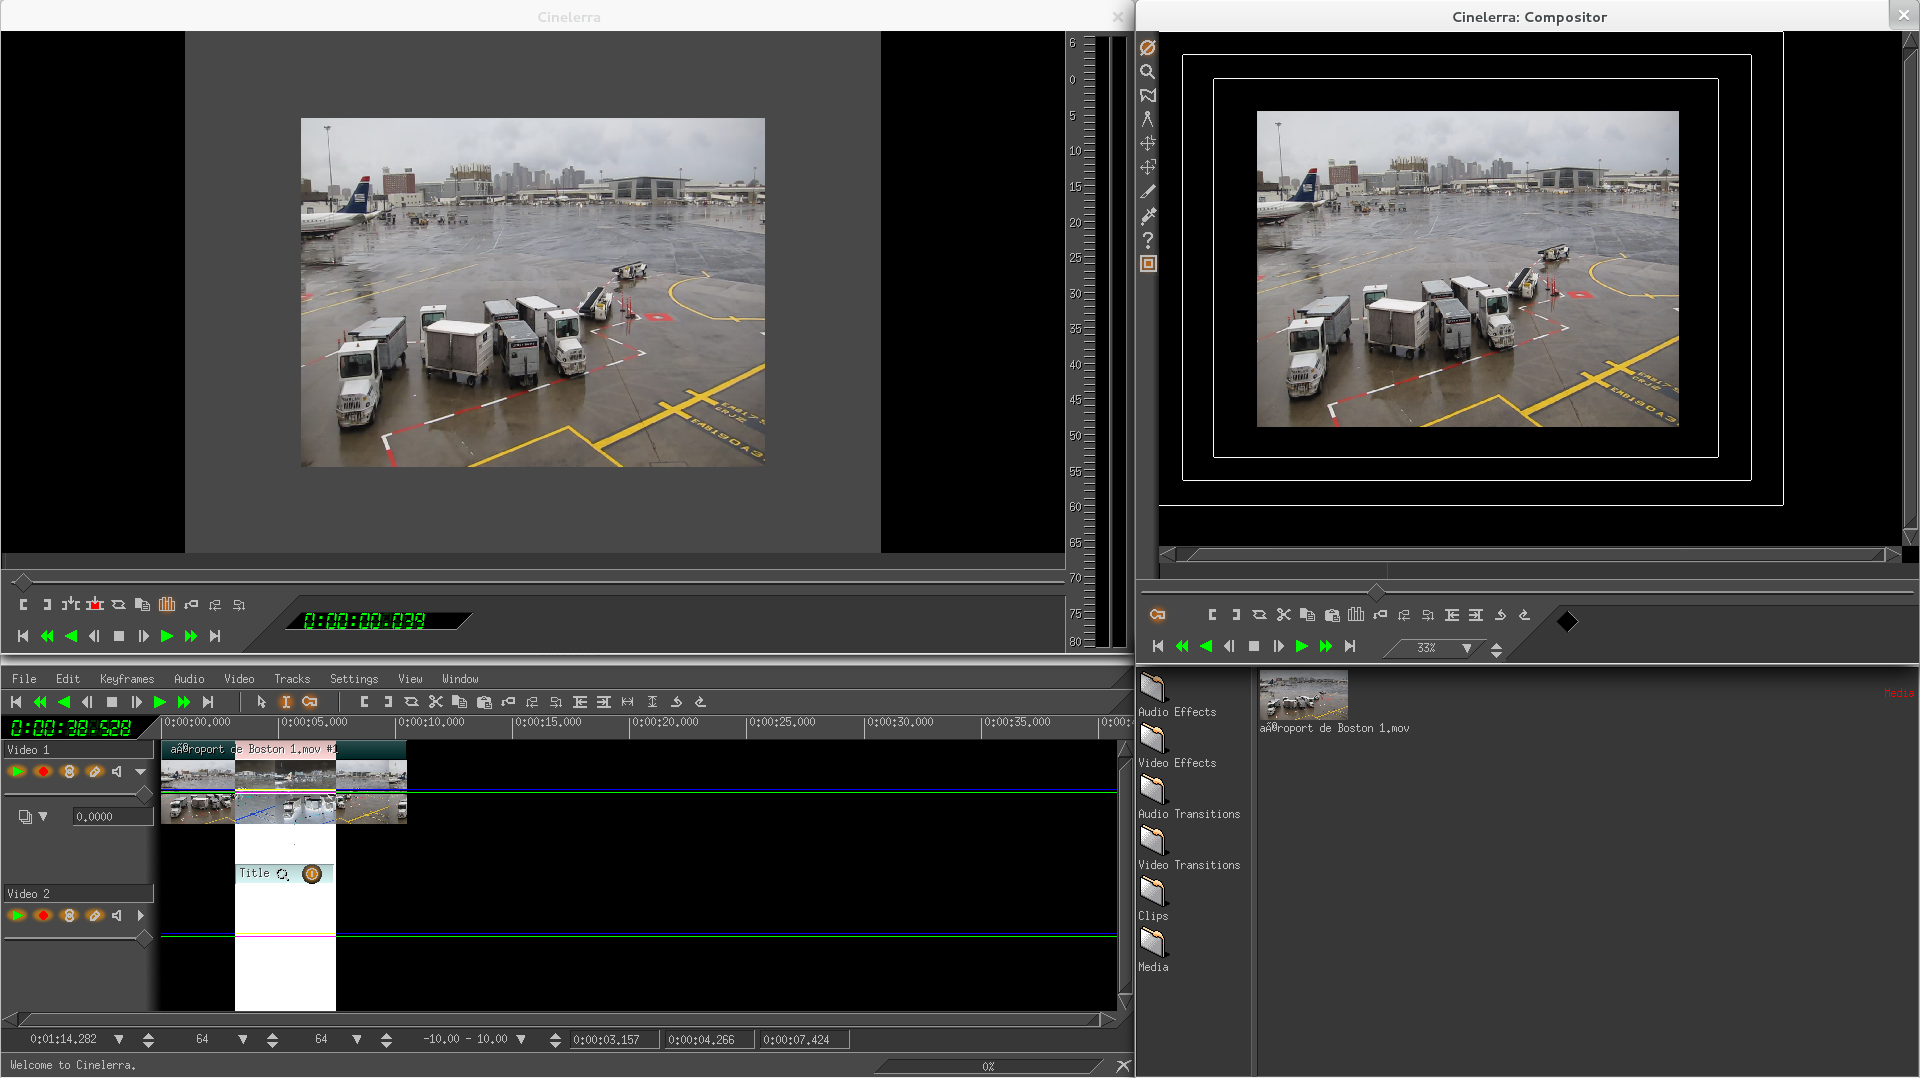
\includegraphics[width=0.95\textwidth]{images/cinelerra}

  \end{center}

  \caption{Interface graphique de cinelerra}

  \label{Yes}

\end{figure}

\paragraph{Structure de l'interface graphique:}

L'interface graphique de cinelerra est composée de quatre fenêtres
principales:

\begin{itemize}
  \item {La timeline (en bas à gauches sur le screenshot): cette
    partie permet de gérer un grand nombre d'opérations sur le contenu
    de la timeline.}

  \item {La fenêtre de ressource (en bas à droite sur le screenshot):
    dans cette fenêtre l'utilisateur peut accéder au différents
    footages qu'il a importé. Il peut aussi accéder au différent
    effets, transitions\ldots}

  \item {Le fenêtre de preview (en haut à gauches sur le screenshot):
    cette fenêtre permet la prévisualisation des footages avant de
    les importer dans la timeline}

  \item {La fenêtre de composition (en haut à droite sur le screenshot):
    cette fenêtre permet d'effectuer des opérations sur les vidéos
    et de prévisualiser la timeline.}

\end{itemize}

\paragraph{}

Cette interface est assez confuse, et ca prise en main n'est pas facile.
Par exemple, pour ajouter des titre ou générique, il faut ajouter
des effets et les configurer. Celà n'est absolument pas intuitif, et
l'ergonomie de cinelerra laisse à désirer. Celà et le fait que le code
n'est absolument pas commenter, et est très difficile à appréhender
explique bien le fait que Cinelerra n'est pas réussi à rassembler les
utilisateurs et développeurs standard de logiciel libre.

\subsubsection{Edition non linéaire}

\paragraph{Conception}

\subparagraph{}

Dans Cinelerra, l'interface utilisateur et la logique de l'édition
vidéo sont deux parties intégralement interdépendante. Au sein du
code, il n'est pas possible de savoir quelle partie est plutôt liée
à l'interface graphique et quelle partie réalise les calculs. Ceci
est dû à sa conception monolithique, les développeurs n'ont pas
pris la peine de dissocier ces deux parties qui sont conceptuelement
complètement différentes.

\paragraph{Accélération materiel}

\subparagraph{}

Lorsque openGL\index{openGL} est présent sur le système, Cinelerra
est en mesure de l'utiliser directement, dans la mesure où cette
fonctionnalité ait été activée lors de la compilation.  La fonction
de compositing est ainsi accélérée, ainsi que la gestion des effets
vidéo openGL.

\subsection {Kdenlive}

Comme précédemment énoncé, Kdenlive utilise le framework orienté
montage et broadcasting MLT\index{MLT}. Dans cette partie, nous allons
dans un premier temps analyser ce framework.

\subsubsection {Framework multimedia orienté montage: MLT\index{MLT}}

\paragraph {Panorama de la technologie} %Overview?

\subparagraph{}

Le framework MLT\index{MLT} est écrit en C et offre une API\index{API}
stable simple et minimaliste. Il est basé sur aucun library (seulement
POSIX)

\glossary {name={POSIX}, description={POSIX est le nom d'une famille
de standards définis depuis 1988 par l'Institute of Electrical and
Electronics Engineers et formellement désignée IEEE 1003. Ces standards
ont émergé d'un projet de standardisation des API des logiciels
destinés à fonctionner sur des variantes du système d'exploitation
UNIX. Il s'agit de la standardisation des API des systèmes communément
appelé UNIX. Source: Wikipedia}} et le standard C, C99). MLT\index{MLT}
bien qu'écrit en C, utilise le paradigme de la programmation orienté
objet en implémentant en interne le concept d'objet. Ce framework
est modulaire, et conçu pour permettre le développement de nouveaux
composants. Il permet l'utilisation des différents core des processeurs
pour faire les calculs, afin d'utiliser au mieux les processeurs
modernes. Il est aussi cross platform et peut être utilisé sur les
principaux systèmes d'exploitation: Linux, BSD, OS X et windows.

\subparagraph{}

MLT\index{MLT} est distribué sous licence LGPL Version

\paragraph{Concepts de base}

\subparagraph{Réseau de service}

\subparagraph{}

Le framework MLT\index{MLT} est basé sur le concept de réseau de service
sur lequel on distingue trois entités (classes) clés: producteur, filtre
et consommateur. Ces différentes classes sont toutes des sous-classe
de la classe appelé ``service``.

On peu schématiser le concept de réseau de service le plus simple de
la manière suivante:

\begin{figure} [H]

  \begin{center}

    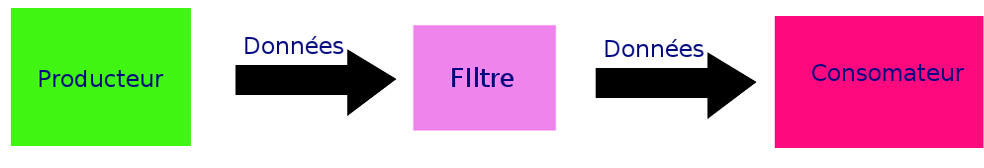
\includegraphics[width=0.95\textwidth]{images/producerConsumer}

  \end{center}

  \caption{Schéma du concept de producteur, filtre, consommateur}

  \label{Yes}

\end{figure}

Le producteur a pour rôle de produire des données (lire un fichier
audio, vidéo\ldots) et de les faire passer au consommateur qui lui est
connecté. Le consommateur a pour but de faire passer ces données (output
datas) à la carte son, device vidéo, un autre fichier, où retransmettre
à travers d'un moyen de télécommunication (broadcasting).  Le filtre
qui n'est pas obligatoire pour lire des donnés multimedias, permet de
modifier les données (par exemple produisant un effet vidéo/audio),
il peut aussi être connecté à plusieurs producteurs, avec comme
exemple la production d'une transition entre ceux-ci.

\subparagraph{}

Mais cela ne permet pas la creation d'éditeur de vidéo non linéaire,
mais seulement la lecture et création de fichier. Pour permettre cette
fonctionnalité, la classe multitrack a été mise en place. Celle-ci
permet de gérer plusieurs producteurs et filtres les uns à la suite des
autres. La multitrack contient plusieurs producteurs et les dispose les
uns à la suite des autres. Ces mêmes producers peuvent aussi provenir
d'une playlist qui est un concept différent, et celles-ci peuvent aussi
être ajoutées directement à un multitrack, et enregistrées sous
forme de fichier de playlist (dans les différents standards existants).

\subparagraph{}

Grâce à la création de ces réseaux de service, il est possible de
créer des timelines complexes, et ainsi créer des logiciels d'édition
vidéo non linéaires. On peut donc schématiser les réseaux de services
de la manière suivante:

\begin{figure} [H]

  \begin{center}

    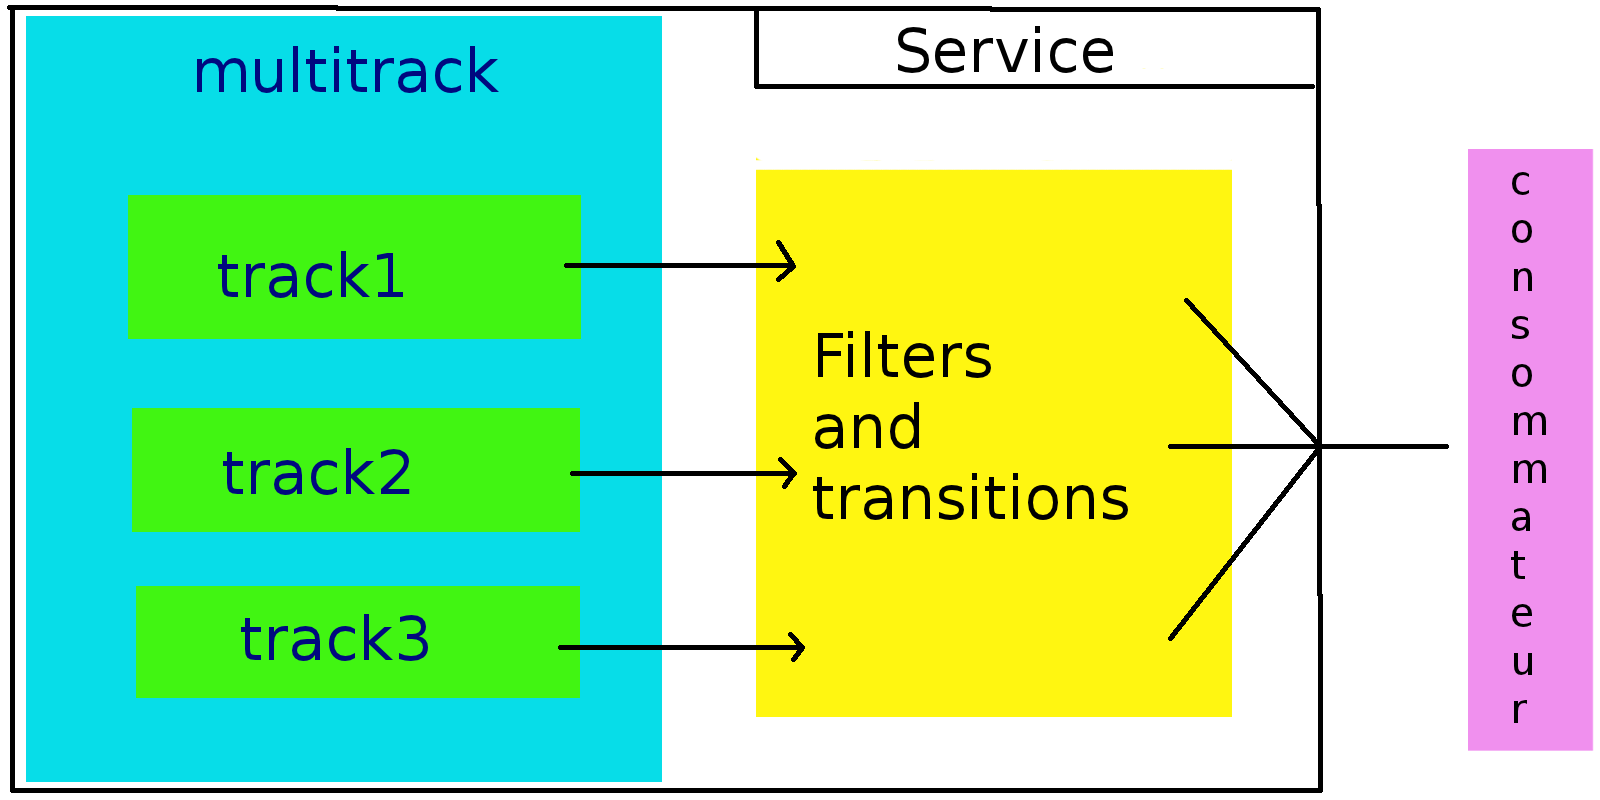
\includegraphics[width=1.0\textwidth]{images/service}

  \end{center}

  \caption{Schéma simplifié d'un service MLT\index{MLT} (point de vu
  interne et
    non utilisateur du framework)}

  \label{Yes}

\end{figure}

\paragraph{Modularité}

\subsubsection{Documentation du code}

\subparagraph{}

Mlt possède une documentation accessible en ligne qui permet de connaitre
les différents services existants. Le code est plutôt bien documenté,
chaque fonction de l'API possède une description. Aussi, des documents
texts dans les source (dossier docs/) permette au développeurs d'avoir un
aperçu de la technologie. De plus il existe un outil en ligne de commande
(melt) qui permet de tester de manière simple le framework. Le gros
soucis étant qu'il est difficile de trouver une documentation claire de
toute l'API, celle-ci ne semble pas être généré automatiquement lors
de la compilation. Dans les sources de MLT\index{MLT}, il n'existe pas
vraiment d'exemple expliquant chacune des fonctionnalités une par une,
il faut pour cela regarder le code de melt, qui permet d'avoir un aperçu
de comment utiliser l'API comme elle a été pensé par les développeurs.

\subparagraph{}

Dans MLT\index{MLT}, les de producteur, consommateurs où filtres sont
des classes extern implémenté sous form de plugins. Certains sont
implémentés directement dans MLT\index{MLT} tel que :

\begin{itemize}

  \item {Le filtre ``transition'': permet la création de transition}

  \item {Le filtre mono: permet de convertir un flux audio en mono}

  \item {Le filtre resize: Permet de redimensionner une vidéo}

  \item {\ldots}

\end{itemize}

Cela est fait grace à des libraries externes en implémentant des
modules externes afin de faire le lien (wrapper)

\glossary{name={adapter}, description={Il permet de convertir l'interface
d'une classe en une autre interface que le client attend. L' Adaptateur
fait fonctionner ensemble des classes qui n'auraient pas pu fonctionner
sans lui, à cause d'une incompatibilité d'interfaces. Source:
Wikipedia}} entre ces librairies et l'API\index{API} précédemment
présenté. Les principales libraries actuellement utilisables à travers
de ce framework sont:

\begin{itemize}

  \item {libav, libdv et libvorbis pour ce qui concerne des codecs et
  muxers/demuxers}

  \item {frei0r pour les effets vidéos}

  \item {ladspa pour les effets audios}

  \item {\ldots}

\end{itemize}

\subparagraph{}

Ces différents services disponibles permettent de lire un nombre
considérable de formats multimedia, en particulier grâce à libav,
et d'effectuer de très nombreuses operations principalement grâce aux
plugins frei0r pour la vidéo et ladspa pour l'audio.

\paragraph{Gestion des services}

\subparagraph{Le ``repository``}

Pour connaitre les différent services présents sur le système,
l'utilisateur a à sa disposition une classe Repository. Celle-ci offre
une API\index{API} simple listant les différents services par type
(consommateur, producteur ou filtre).  Pour illustrer, le simple code
suivant permet de récupérer la liste de tous les effets présents sur
le système:

\subparagraph{}

\begin{lstlisting}
  mlt_repository repo = mlt_repository_init (NULL) /* We just use the
  standard module path */ mlt_properties filters = mlt_repository_filters
  (repo); /*
\end{lstlisting}

\subparagraph{Les ``factory''} Dans le but de simplifier la création de
services de différents types, MLT\index{MLT} utilise le design pattern
de la factory. On peut ainsi créer n'importe quel type de service de
manière simple en utilisant les différentes factories existantes. Bien
que tous les objets d'un réseau de service soient des descendants de
la classe Service, les développeurs ont décidé de créer 4 méthodes
différentes de la classe factory:

\begin{itemize}

  \item {mlt\_factory\_producer: permet d'instancier des producteurs}

  \item {mlt\_factory\_filter: permet d'instancier des filtres}

  \item {mlt\_factory\_transition: permet d'instancier des transitions}

  \item {mlt\_factory\_consumer: permet d'instancier des consommateurs}

\end{itemize}

\subparagraph{}

Par exemple, pour créer un effet ``invert'' depuis MLT\index{MLT}
il suffit de faire:

\subparagraph{}

\begin{lstlisting}
  filter = mlt_factory_filter ( "invert", "my-invert-effect");
\end{lstlisting}

Il sera ensuite possible d'ajouter ce service au réseau de service.

\subparagraph{Les données dans un réseau de services}

\subparagraph{La classe Frame}

\subparagraph{}

Les données qui transitent dans un réseau de service sont contenues dans
des objets de type frame. Celles-ci contiennent à la fois les données
audio et les données vidéos. Les producteurs peuvent setter ces données
grâce aux méthodes mlt\_frame\_set\_audio et mlt\_frame\_set\_video.

\subparagraph{Relations entre les différents services en terme de flux
de données}

Afin commencer le flux de données dans un réseau de service, le
consommateur est celui qui fait la demande de donner (pull datas) les
données depuis le service sur lequel il est connecté. Les autre services
réagissent en fonction,et forment une chaine jusqu'au producteur qui
produit les données, et les fait suivre au service suivant et ainsi de
suite. Ce processus peut être schématisé de la manière suivante:

\begin{center}

  \begin{tabular}{ | c | c | c | c |}

    \hline

Phase & producteur & Filtre & Consommateur    \\ \hline \hline

1 & & & Request frame   \\ \hline

2 & & Réception de la demande & \\

  & & Demande la frame à son tour & \\ \hline


3 & Réception de la demande & & \\

  & Génération de la frame à la position & & \\

  & Mise à jours de la position & & \\

  & Mise à disposition de la frame & & \\ \hline

4 & & Réception de la frame       & \\

  & & Update de la frame & \\

  & & Mise à disposition & \\ \hline

5 & & & Réception et    \\

  & & & process de      \\

  & & & la frame        \\ \hline

  \end{tabular}

\end{center}

\subparagraph{}

Cette manière de fonctionner implique que seul le consommateur est
le moteur du réseau. Il est celui qui doit faire partie d'un thread
séparé et les appels à la fonction get\_frame doivent être faits
dans une boucle principale.  Ces appels s'arrêteront au moment où le
flux a été terminé (EOS).


\paragraph{Accélération materiel}

\subparagraph{}

Au niveau de l'accélération materiel, MLT\index{MLT} supporte le
decoding avec acceleration matériel pour les cartes graphiques Nvidia
\glossary{name={Nvidia}, description={Nvidia Corporation est l'un des plus
grands fournisseurs de processeurs graphiques, de cartes graphiques et de
chipsets pour PC et consoles de jeux}} (via VDPAU), et pour l'affichage
mais pas le compositing vidéo accéléré.

\glossary{name={VDPAU}, description={VDPAU (Video Decode and Presentation
API for Unix) est une bibliothèque open source (libvdpau) et une
interface de programmation conçus par NVIDIA initialement pour ses
cartes graphiques GeForce 8 et ses derniers processeurs graphiques. Cette
interface permet à des programmes de vidéo de décharger de la mémoire
des parties du processus de décodage de vidéo et de son traitement
aval vers le processeur graphique.}}

\paragraph{Fonctionnalités haut niveau (High level features)}

\subparagraph{}

La petite API qu'offre ce framework comporte des méthodes et des
fonctions haut niveau et permet de répondre à des besoins spécifiques
de l'édition vidéo de manière simple pour l'utilisateur.

\subparagraph{Génération de waveform/thumbnail depuis une frame}

\subparagraph{}

Le framework offre par example une fonction permettant la génération
(sous forme d'image) des waveform de la partie audio d'une frame, et
de thumbnail depuis la partie audio.  Dans la partie précédente, nous
avons constaté que la visualisation avancée de chaque frame était une
fonctionnalité très utile en particulier dans le cadre de la création
de films.

\subparagraph{Serialization et deserialization de projets}

\subparagraph{}

Il intègre un système de serialisation, deserialization, ce qui permet
de sauvegarder facilement les projets, avec les différents tracks,
effets, transition\ldots dans le cadre d'application de montage vidéo.

\subparagraph{}

Le framework MLT\index{MLT} offre des bindings haut niveau pour les
languages: C++, C\#, Java, Lua, Perl, PHP, Ruby, TCL et Python. Cela
permet à un plus grand nombre de développeurs d'envisager
l'utilisation de MLT\index{MLT} dans leurs applications. C'est grâce
aux bindings C++ que Kdenlive a pu être développé au dessus du
framework\index{framework} MLT\index{MLT}

\paragraph{Fonctionnalités}

\subparagraph{ }

Cette analyse technique du projet MLT\index{MLT} nous permet de constater
que son fonctionnement est simple, et son API petite, et facile à
prendre en main.  Il permet de répondre à différents besoins de base
des professionnels en terme de fonctionnalités:

\begin{itemize}

  \item {Ajout de titres et génériques: A travers du module développé
  par la
    communauté Kdenlive: QImage.}

  \item {Gestion des keyframes: possible dans les modules implémentant
    cette fonctionnalité, pas de solution générique au niveau du core
    de MLT\index{MLT}}

  \item {Visualisation image par images et waveform: Directement
  accessible à
    travers du core de MLT\index{MLT}.}

  \item {Visualisation image par image et waveform: Directement
  accessible à
    travers du core de MLT\index{MLT}.}

\end{itemize}

\subparagraph{}

La principale lacune en terme de fonctionnalité est l'impossibilité de
faire du time remapping, mais il est tout de même possible de gérer
le contrôle de la vitesse de lecture des clips, ce qui est un point
essentiel.

\subsubsection {Logiciel de montage vidéo basé sur MLT\index{MLT}:
Kdenlive}

\subparagraph{}

Kdenlive est l'éditeur vidéo créé par la communauté en charge
du bureau libre KDE. Ce logiciel est donc écrit en C++ utilisant le
framework graphique QT \glossary{name={QT}, description={framework
orienté objet et développé en C++ par Qt Development Frameworks,
filiale de Nokia. Il offre des composants d'interface graphique (widgets),
d'accès aux données, de connexions réseaux, de gestion des fils
d'exécution, d'analyse XML, etc. Qt est par certains aspects un framework
lorsqu'on l'utilise pour concevoir des interfaces graphiques ou que l'on
architecture son application en utilisant les mécanismes des signaux
et slots par exemple.}} ainsi que les kdelibs qui forment le framework
permettant la création d'application intégré au bureau du même nom.
L'analyse technique de ce logiciel n'a pas vraiment d'intérêt car on
est en présence d'une interface graphique tirant partit du framework
MLT\index{MLT}.

\paragraph {Capture d'écran}

\subparagraph{}

\begin{figure}[H]

  \begin{center}

    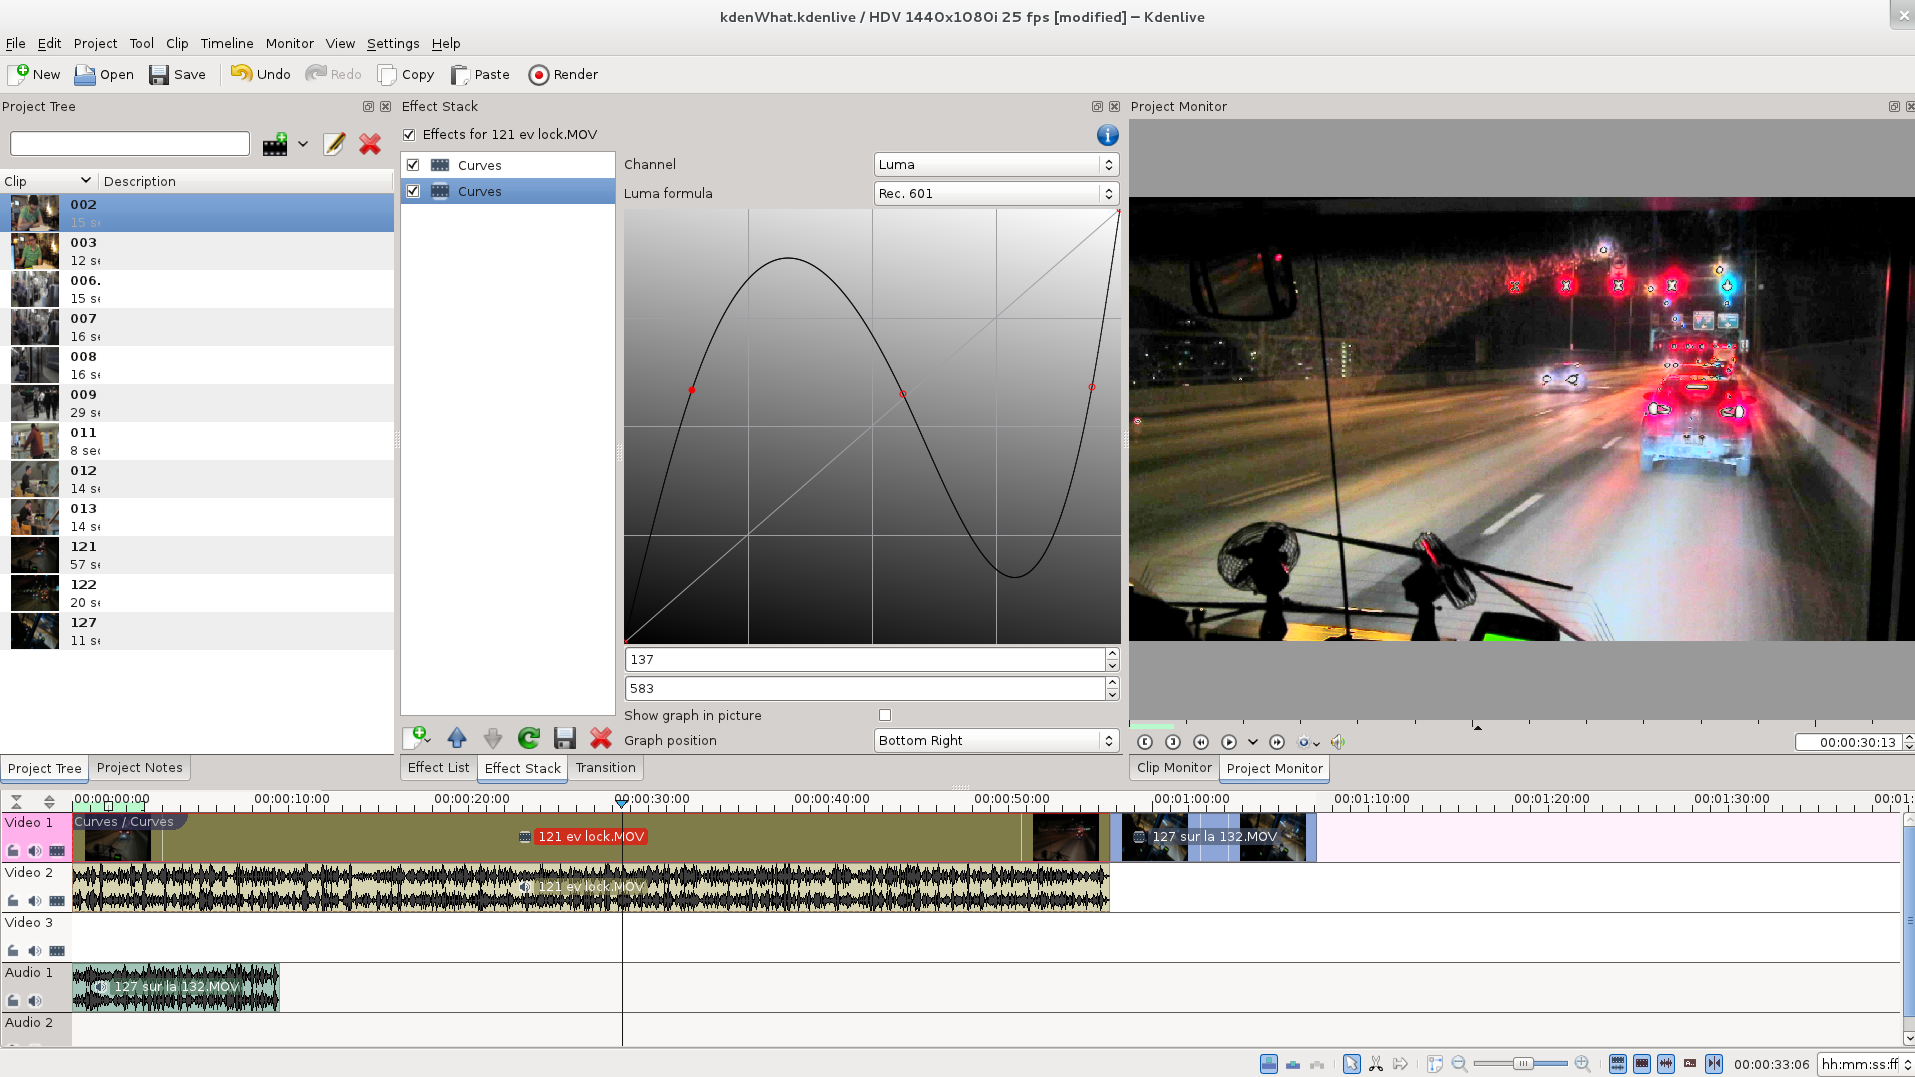
\includegraphics[width=0.95\textwidth]{images/kdenlive}

  \end{center}

  \caption{Screenshot de Kdenlive}

  \label{Yes}

\end{figure}

L'interface graphique de Kdenlive est composé d'une seule fenêtre
présentant quatre éléments majeurs:

\begin{itemize}

  \item {La timeline en bas}

  \item {La gestion des footages, en haut à gauches}

  \item {La gestion des effets et transitions, au centre en haut. La
  configuration de ceux-ci se fait dans cette même partie.}

  \item {Le previewer, en haut à droite}

\end{itemize}


Ce screenshot montre que Kdenlive présente de nombreuses fonctionnalités
à l'utilisateur bien que son interface soit assez épuré.

\subsection {PiTiVi}

Comme précédemment énoncé, PiTiVi utilise le framework multimedia
GStreamer. Dans cette partie, nous nous concentrerons sur l'analyse de
ce framework.

\subsubsection {Framework multimedia: GStreamer}

\paragraph {Panorama de la technologie} \subparagraph{}

GStreamer un framework multimedia basé sur le concept de pipeline
écrit en C.  L' API de ce framework est plus complet que celle de
MLT\index{MLT} puisque les use-cases auxquels celui- ci cherche à
répondre sont plus nombreux. En effet, la communauté GStreamer a pour
objectif de créer un framework open source permettant de répondre au
plus grand nombre possible de cas d'utilisations ayant un lien avec le
multimedia (depuis les téléphones mobiles jusqu'aux renders farms
en passant par les logiciels de montage video).  Ce framework, bien
qu'écrit en C, utilise le paradigme objet, à travers de la librairie
Glib. Cette librairie implémente de nombreuses API et en particulier
la notion d'objet en C grace au module GObject. La Glib permet aussi
la gestion des threads, des signaux\ldots De très nombreux projets
de logiciels libres l'utilisent, en particulier le projet d'interface
graphique Gnome. GStreamer offre une API stable aussi bien pour les
développeurs de plugins que pour les développeurs d'applications. Il
est hautement multi threaded\glossary{name={thread}, description={Il
s'agit de la plus petit unité de processus qui peut être exécutée
par un système d'exploitation. Ils permettent à un même ``programme'',
processus d'exécuter du code de manière concurrente.}}, et est thread
safe, c'est a dire que la mémoire partagée par les différents threads
ne peut pas être corrompue dans le cas ou plusieurs threads voudraient
la modifier en même temps(en utilisant le système d'exclusion mutuel).

Le schéma suivant permet de représenter graphiquement l'architecture
globale du framework:

\begin{figure}

  \begin{center}

    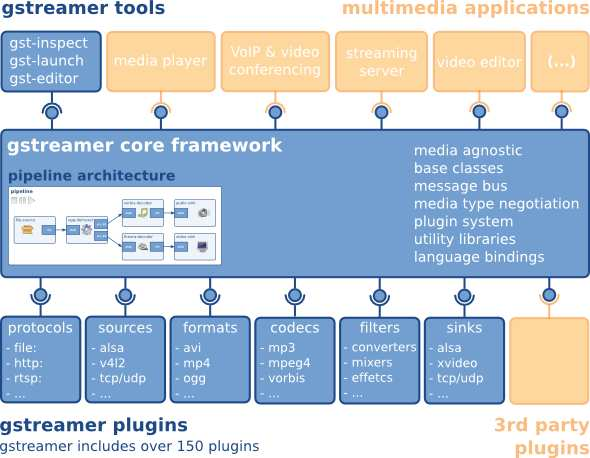
\includegraphics[width=0.70\textwidth]{images/gstoverview}

  \end{center}

  \caption{Architecture du framework GStreamer}

  \label{Yes}

\end{figure}

\subparagraph{}

GStreamer est distribué sous licence LGPL Version

\subsubsection{Documentation du code}

\subparagraph{} Gstreamer utilise la syntaxe de gtk-doc afin de
permettre la génération automatique de la documentation à partir du
code source. Celà signifie que l'API est complètement documenté et
accessible sur internet. Afin de permettre d'obtenir des information
sur les différent éléments, un outil gstreamer a été développé
(gst-inspect). Il existe aussi des livres libres (pas toujours actualisé)
permettant d'aider les développeurs soit à développer des applications
en utilisant GStreamer (Gstreamer manual) où des plugins/éléments
(Plugins Writer Guide).  Il est aussi possible de créer des pipeline en
ligne de commande grace à l'outil 'gst-launch'.  En terme d'exemple,
les développeurs essaye de tenir à jours des example pour chaque API
nouvellement créé, mais cela n'est pas toujours le cas.

\paragraph{Concepts de base}

\subparagraph{Le concept de pipeline}

\subparagraph{}

La grande majorité des classes dans GStreamer dérive de la classe
GstElement qui est l'élément de base dans un pipeline, lui même
GstElement. Un schéma permet d'expliquer cette notion de pipeline
assez facilement:

\newpage \begin{figure} [H]

  \begin{center}

    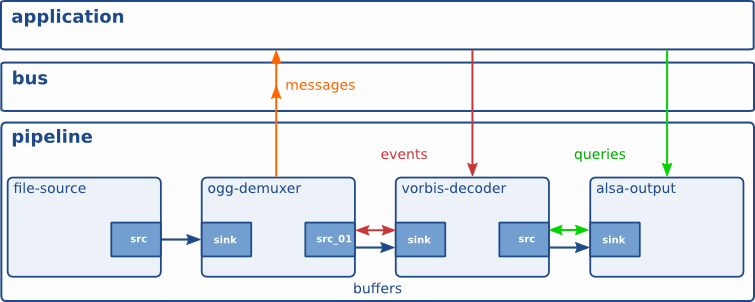
\includegraphics[width=0.95\textwidth]{images/gstpipeline}

  \end{center}

  \caption{Un pipeline GStreamer permettant la lecture d'un fichier
  audio ogg
    ayant pour codec vorbis (ce schéma prend en compte d'autres notions
    importantes du framework).}

  \label{Yes}

\end{figure}

\subparagraph{}

On constate que l'architecture est assez similaire à celle
MLT\index{MLT}, avec pour grande difference le fait que les éléments
composants le ``réseau de service'' sont tous dans un même élément:
le pipeline. Cet élément GStreamer execute un thread séparé à
partir du moment où l'on cherche a jouer son contenu. Dès lors,
les données transitent entre les différents élément gstreamer, a
commencé par l'élément source. Dans l'exemple donne par ce schéma,
il s'agit d'un file-source, et terminant par le sink, dans notre exemple
alsa-output. Les éléments entre les deux se chargent du demuxing
(ogg-demux), et du decoding (vorbis-decoder).

\subparagraph{}

Une autre différence réside dans le fait que l'utilisateur de GStreamer
a un contrôle plus important que dans le cas de MLT\index{MLT} sur
les composants de la chaines d'éléments permettant la reproduction de
contenu multimedia.  Dans GStreamer chaque tâche est effectuée par un
élément, c'est à dire qu'un service MLT\index{MLT} sera décomposé
en plusieurs élément GStreamer. Dans le cadre d'un producteur en
particulier, chez GStreamer, cela est effectué à travers un élément
pour chaque étape du coding/decoding/muxing/demuxing, et dans certain
cas, du parsing du bitstream. Cette décomposition en petits éléments
effectuant une tâche a le gros avantage de permettre la réutilisabilité
de chacun d'eux et ce, dans les différents  contextes d'applications
multimédia.

\subparagraph{Communication entre les éléments}

\subparagraph{}

La communication entre ces différents éléments se fait au travers des
GstPad. Il convient de représenter un élément (dans ce cas un demuxer,
qui permet de recevoir un flux en entrée de le décomposer afin d'avoir
deux sorties, l'une contenant les données audios, et l'autre avec les
données vidéos), de la manière suivante:

\begin{figure} [H]

  \begin{center}

    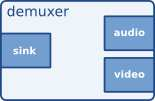
\includegraphics[width=0.30\textwidth]{images/gstdemuxer}

  \end{center}

  \caption{Représentation graphique d'un GstElement permettant le
  demuxing.}

  \label{Yes}

\end{figure}

Sur ce schéma, on constate la présence d'un sink pad, nommé ``sink'',
et deux source pad, nommé ``audio'' et ``video''. Ces objets (GstPad),
permettent la connection entre les différents élément. Il peuvent être
comparé au ``prise'' et ``port'' dans le monde réel.  Afin de brancher
une prise dans un port, il convient de s'assurer que ceux-ci soient
compatibles, c'est ce rôle qu'ont les caps, assurer la compatibilité
de la communication entre différents éléments.

\paragraph {Modularité}

\subparagraph{}

GStreamer est extrêmement modulaire, et l'on peut l'étendre facilement
en créant de nouveaux éléments. Il suffit d'ajouter ces élément
(sous forme de plugins) sur le système pour que l'utilisateur puisse
tirer partie des nouvelles fonctionnalités. La communauté GStreamer
offre des collections de plugins contenant un très grand nombre
d'élément. Ces set de plugins sont classés selon des critères précis:

\begin{itemize}

  \item {base: Plugins de grande qualité et très bien maintenus. Il
  offre aussi
    des classes de base afin de faciliter la creation d'éléments.}

  \item {good: Plugins de qualité, ayant une licence LGPL}.

  \item {Ugly: Plugins de qualité, ayant des problèmes au niveau de
  la licence.}

  \item {bad: Plugins de moins grande qualité, ayant des problèmes
  au niveau
    de la licence. Il s'agit d'éléments dont le code a été moins
    testé et risque ainsi de présenter davantage de bugs.}

\end{itemize}

\subparagraph{}

De nombreuses librairies sont wrapper dans ces différentes collections
de plugins, par exemple, dans ``bad'', les librairies d'effets ladspa et
frei0r y sont incluses et dès qu'elles sont installées sur le système,
elles permettent à n'importe quelle application basée GStreamer de
bénéficier de leurs fonctionnalités.  Ces plugins sont distribués
sous forme de librairies partagées, et peuvent donc être chargées à
la volée, durant l'exécution du framework.

\subparagraph{}

En terme de lecture de contenu multimedia, les développeurs GStreamer
conseillent l'utilisation de la collection de plugins ``gst-ffmpeg''
qui permet de bénéficier de toutes les codec, muxer et demuxer de
cette librairie. D'autres librairies tel que libogg, libdv, x264\ldots
sont wrapper dans les différentes collections de plugins précédemment
présentées.

\paragraph{Gestion des éléments}

\subparagraph{}

La gestion des éléments est très comparable à ce qui est fait dans le
framework MLT\index{MLT}, c'est à dire, que l'on a une classe GstRegistry
(comparable à la classe repository de MLT\index{MLT}), et des GstFactory
qui permettent la fabrication facile d'éléments.

%DIMANCHE SOIR

\paragraph{Accélération materiel}

\subparagraph{}

A l'heure actuel, il existe des éléments permettant le decoding de
vidéo en utilisant, l'accélération materiel pour les carte graphiques
Nvidia et Intel. Cela n'est pas activé par default mais les développeur
travail actuellement sur ce problème, et cela devrai être activé par
default très prochainement. De plus, il est techniquement pas possible
dans la version actuel de permettre le compositing accéléré par
matériel. Celà est du au fait que les éléments dans un pipeline n'est
pas la possibilité de ``communiquer'' entre eux, et par concéquent,
de laisser l'élément un élément qui pourrai tirer partie de
l'accélération materiel faire l'opération de compositing. Afin de
résoudre ce problème, les développeurs de GStreamer, ont mis en place
un système permettant d'ameliorer la communication entre les éléments
dans la version 1.0 qui doit sortir avant la fin de l'année. Afin de
s'assurer que le problème soit résolu dans tout les cas (c'est à dire
lors de la reproduction aussi bien que du rendering), il faudra très
probablement développer un élément glcomposition.

\paragraph{Et l'édition vidéo?}

\subparagraph{}

En effet, tout cela ne nous permet pas de faire  de l'édition vidéo
requiert la création de pipeline dynamique, c'est à dire qui permet
de faire évoluer les éléments présents dans le pipeline au fil du
temps.  C'est pour cette raison que les éléments du plugins Gnonlin
ont été développés. Il s'agit de 4 éléments principaux dont voici
la définition

\begin{itemize}

  \item {GnlComposition: élément le plus important qui permet de
  faire évoluer
    le pipeline de manière dynamique}

  \item{Gnl[uri/file]Source: élément source qui a les propriétés
    nécessaires pour savoir à quel moment il doit être présent ou
    non dans le pipeline}

  \item{GnlOperation: élément qui permet l'application d'effet,
  transition
    etc\ldots il a aussi les propriété permettant de savoir à quel
    moment il doit être présent ou non dans le pipeline}

\end{itemize}

\subparagraph{}

Mais ces éléments ne permettent pas de facilement créer des application
de montage audio/ou vidéo. Le core actuel de PiTiVi utilise directement
ces élément afin de gérer les notion propre à l'édition vidéo,
mais les développeur se sont rendu compte que cela était trop complexe
à utiliser, et par concéquent PiTiVi n'est pas une simple interface au
dessus de GStreamer, mais introduit de plusieurs concepts supplémentaires
au dessus de ces éléments.

\paragraph{}

Et plus récemment, les développeurs de GStreamer ont décidé de créer
une nouvelle librairie basé sur GStreamer permettant de faciliter
au maximum la création d'un logiciel d'édition vidéo basé sur
GStreamer: gst-editing-services.  L'objectif premier de cette librairie
est d'implémenter les concepts même d'édition vidéo directement dans
le backend. C'est à dire qu'au cœur de cette librairie, on retrouve
les concepts de timeline, de layer, de transition, d'effets\ldots Mais
bien évidemment, celle-ci étant basée sur GStreamer, le concept
the pipeline continu d'exister, et il est très facile de créer un
pipeline directement depuis une timeline. Un schéma permettant de
montrer les concepts de base de cette librairies permet de simplifier
la compréhension de son fonctionnement.

\begin{figure} [H]

  \begin{center}

    \includegraphics[width=1.0\textwidth]{images/ges}

  \end{center}

  \caption{Concepts introduits par GES}

  \label{Yes}

\end{figure}

Ce schéma permet de representer graphiquement les différents concepts
qui entre en jeux. Niveau utilisateurs, l'API\index{API} de GES peut être
utiliser de manière plus où moins avancé. C'est à dire que dans le
cadre d'application simple d'édition vidéo, la notion de média est
caché à l'utilisateur et celui-ci ne s'intéresse simplement à ce
que sont les fichiers, effets etc\ldots Mais il est possible de faire
une utilisation avancé de cette API afin de créer un éditeur vidéo
à visée professionnel.

\subparagraph{}

Tout comme ce que l'on a pu constater dans MLT\index{MLT}, GES
offre des fonctionnalités de haut niveau tel que la génération de
thumbnails à partir de la timeline, la serialisation, deserialization
des timelines\ldots

\subparagraph{}

Dans les faits, GES est très comparable à ce qu'est le core actuel
de PiTiVi. C'est donc naturellement que PiTiVi est en train de faire la
migration vers les gst-editing-services.

\paragraph{Fonctionnalités}

\subparagraph{ }

Cette analyse technique du projet GStreamer et GES nous permet de voir
que GStreamer étant une technologie très complexe, les développeurs
ont développé diverse outils afin de permettre la création de manière
simplifié de logiciels de montage vidéo. Ce framework à tracer de GES
permet de répondre aux différents besoins de base des professionnels
en terme de fonctionnalités:

\begin{itemize}

  \item {Ajout de titres et génériques: GES offre des TextLayer et
  TitleSource
    qui permettent d'ajouter des titres de manière simple, en ce qui
    concerne les générique, cela est possible à travers de keyframes,
    mais cela n'est pas vraiment supporté à l'heure actuel. Il s'agit
    d'un manque majeurs pour répondre aux besoins des professionnels}

  \item {Gestion des keyframes: possible dans les modules implémentant
    cette fonctionnalité, pas de solution générique au niveau du core
    de MLT\index{MLT}}

  \item {Gestion des keyframes: Le framework GStreamer offre la
  possibilité
    de créer des keyframes sur toutes les propriétés de ces élément
    à grace à la classe GstInterpollation}

  \item {Visualisation image par image: Directement accessible grace
  à GES.}

\end{itemize}

\subsubsection {Logiciel de montage vidéo basé sur GStreamer: PiTiVi}

\subparagraph{}

PiTiVi est l'éditeur vidéo supporté par la communauté GStreamer et la
communauté Gnome. Il est écrit avec le language de programmation Python,
et la libraries graphique Gtk+ \glossary{name={gtk+}, description={The
GIMP Toolkit est un ensemble de bibliothèques logicielles, permettant
de réaliser des interfaces graphiques. Cette bibliothèque a été
développée originellement pour les besoins du logiciel de traitement
d'images GIMP. GTK+ est maintenant utilisé dans de nombreux projets,
dont les environnements de bureau GNOME, Xfce et ROX.}}.

\paragraph {Capture d'écran}

\subparagraph{}

\begin{figure}[H]

  \begin{center}

    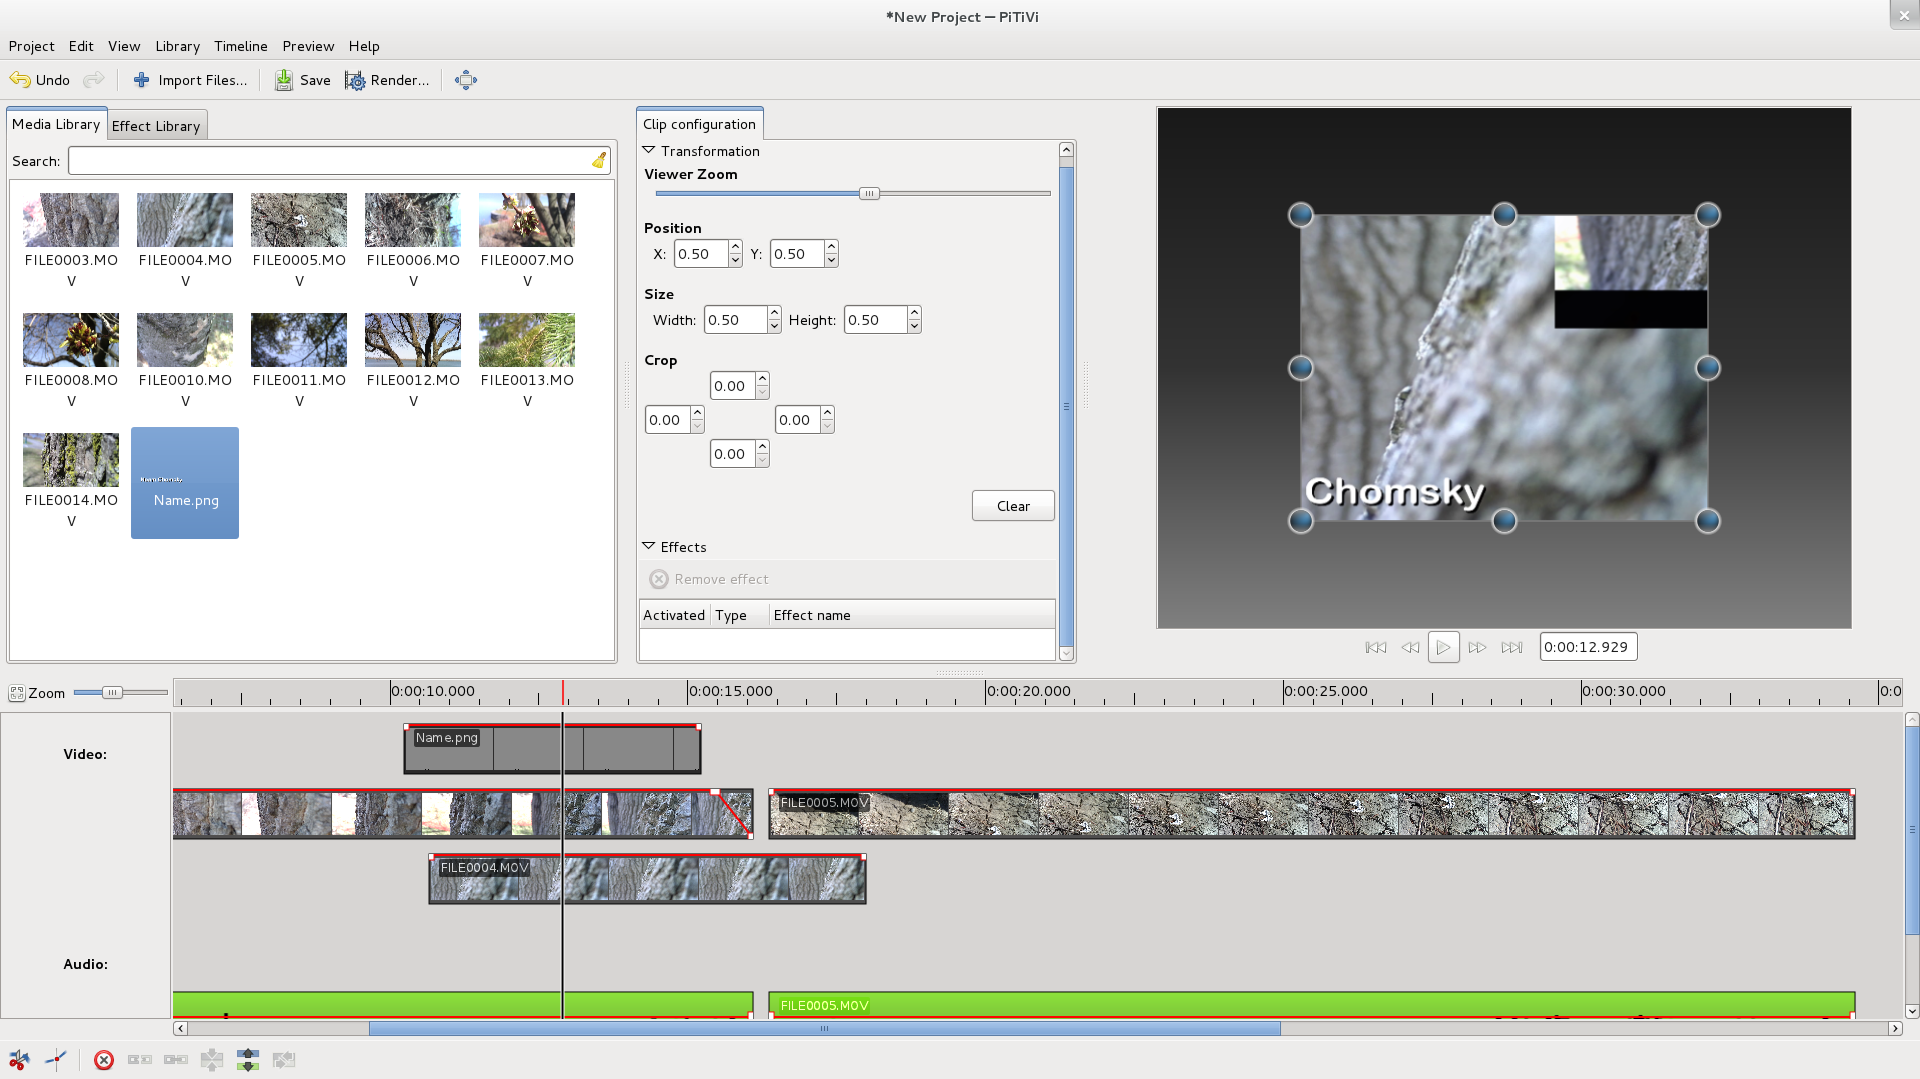
\includegraphics[width=0.90\textwidth]{images/pitivi}

  \end{center}

  \caption{Screenshot de PiTiVi}

  \label{Yes}

\end{figure}

\paragraph{}

L'interface graphique de PiTiVi est aussi composé d'une seule fenêtre
présentant quatre éléments majeurs:

\begin{itemize}

  \item {La timeline en bas}

  \item {La gestion des footages et effet, sous forms d'onglets, en haut
  à gauche}

  \item {La configuration des effets et transformations, au centre
  en haut.}

  \item {Le previewer, en haut à droite}

\end{itemize}

\paragraph{}

Ce screenshot permet de voir l'interface simple et épuré de
PiTiVi. Celà traduit en effet son manque de fonctionnalités, mais aussi
le but des développeurs qui est d'offrir le strict nécessaire en terme
d'interface. C'est à dire offrir les options seulement si celle-ci sont
utiles à l'utilisateur.

\newpage \section{Analyse des communautés}

\paragraph{}

Afin d'analyser une communautés, quatres éléments majeurs sont à
prendre en comptes:

\begin{itemize}

  \item {Le code source: il convient de mesurer le nombre d'auteur,
  la vitesse de son évolution
    d'évolution. Afin de mesurer cela, des outils statistiques
    existent, en particulier pour le système de gestion de code
    source\glossary{name={Système de gestion de version}, description={Un
    logiciel de gestion de versions (ou VCS en anglais, pour Version
    Control System) est un logiciel qui permet de stocker un ensemble de
    fichiers en conservant la chronologie de toutes les modifications
    qui ont été effectuées dessus. Il permet notamment de retrouver
    les différentes versions d'un lot de fichiers connexes. Source:
    Wikipedia}} git\glossary{name={git}, description={Git est un logiciel
    de gestion de versions décentralisée. C'est un logiciel libre
    créé par Linus Torvalds, le créateur du noyau Linux, et distribué
    sous la GNU GPL version 2.}}, et à l'outil gitstats. Celà permet
    d'analyser l'état de santé d'un communauté de logiciel libre.}

  \item {Les entreprises qui travail sur le projet: Les logiciels libre
    font à l'heure actuel actuel pleinement partit de l'économie
    du logiciel informatique. L'implication des entreprises dans les
    différentes communautés libre est un point essentiel qui permet
    permettant de comprendre la viabilité de celui-ci en particulier,
    comme c'est le cas dans cette analyse, au prêt des professionnels}

  \item {Le nombre de bugs rapportés, et l'analyse de la vitesse de fix
    de ceux-ci}

  \item {Communication entre les membres de la communauté}

\end{itemize}

\paragraph{}

Pour les différent projets précédemment analyser, nous allons
faire un état des lieux de leurs communauté selon les deux critère
précédemment mentionnés.

\subsection {Analyse du code source}

\paragraph{}

Afin d'analyser le code, nous avons exécuté le script gitstats sur
les différent repository git des projets:

\begin{itemize}

  \item {cinelerra: version communautaire du projet:
  http://git.cinelerra.org }

  \item {MLT\index{MLT}:
http://www.mltframework.org/gitweb/mlt.git?p=mltframework.org/mlt.git;a=summary}

  \item {GStreamer: http://cgit.freedesktop.org/gstreamer/gstreamer/ }

\end{itemize}

Il est important de noter que ce tableau doit être analyser en prenant
en compte les paramètres suivants:

\begin{itemize}

  \item {Le fait que le projet cinelerra ne soit pas réelement basé
  sur la communauté
    risque de faussé la comparaison avec les autres projets, mais il
    convient de garder en tête que ce projet est le seul projet présent
    sur le marché de l'édition professionnel.}


  \item {Le fait que cinelerra ne soit pas un framework mais une
    application complète d'édition vidéo doit être pris en compte}

  \item {Dans MLT\index{MLT}, les plugins sont prise en compte, alors
  que pour
    GStreamer, on ne prend en compte que le core du famework (qui n'est
    qu'un très petit partie du framework)}

\end{itemize}

\begin{center}

  \begin{tabular}{ | c | c | c | c |c| c |}

    \hline

         &Nombre de& Nombre de & Nombre de&Mois avec& Mois du \\

Logiciel &lignes & développeurs& commits le&le plus grand & premier\\

         &&&mois passé&nombre de&commit\\

         &&&&commits&\\

\hline \hline

Cinelerra&1 064 372 &28&1& Septembre 2006&Juin 2003\\

&&&&(38 commits)&\\ \hline

MLT\index{MLT}& 110011 &12&15& Septembre 2004&Décembre 2003\\

&&&&(53 commits)& \\ \hline

GStreamer& 435 930  &205&47& Décembre 2001&Janvier 2001\\

Plugins-base& 413 883 &46&47& Mars 2004&Décembre 2001\\

Plugins-bad& 696 521 &305&156& Juin 2006&Décembre 2001\\

GES& 51 932 &14&49& Juin 2010&Aout 2009\\

\hline

  \end{tabular}

\end{center}

Ce tableau montre quel le codebase de Gstreamer et de ces plugins est plus
le important. Celà semble tout à fait logique puisque ce framework a
pour objectif de répondre à plus de problème. Il est intéressant de
constater que la communauté MLT\index{MLT} est très petite (seulement
12 développeurs), cela s'explique par le fait que l'API maintenu est
minimalist, et permet de répondre à un problème précis.  Le nombre de
développeur de cinelerra n'est aussi pas très grand, dans les faits, il
s'agit plus où moins d'un ``one man show'', et Adam Williams (employé
Heroine) est responsable de l'immense majorité du code. Le nombre de
commit le mois passé laisse penser que Cinelerra est un projet très peu
actif. Mais celà n'est pas vrai puisqu'en aout dernier, la société
Héroine a encore releasé une nouvelle version contenant quelques
nouvelles fonctionnalités et corrigé quelque bugs assez importants.

\subsection {Analyse des mailing lists}

Cette analyse porte sur les mailing listes officiel des différent
projets:

\begin{itemize}

  \item {cinelerra: version communautaire du projet:
    cinelerra.org/mailinglists.php}

  \item {MLT\index{MLT}: cinelerra.org/mailinglists.php}

  \item {GStreamer: http://gstreamer.freedesktop.org/lists/}

\end{itemize}


\begin{center}

  \begin{tabular}{ | c | c | c | c|}

    \hline

         & Nombre minimum & Nombre maximum & Nombre moyen \\

Logiciel & par mois       & par mois   & par mois \\

\hline \hline

Cinelerra & 20 & 499 & 55 \\

          &  Juin 2011 & Aout 2007 & \\

\hline

MLT\index{MLT} & 37 & 178 & 72 \\

     & Mars 2009 & May 2011 & \\

\hline

GStreamer & 238 & 521 &  387\\

          & Janvier 2010 & Aout 2010 & \\

\hline

  \end{tabular}

\end{center}

D'après l'analyse des mailing lists, on voit une fois de plus que le
projet GStreamer est un projet plus important. Mais les autres projet ont
de gros flux de mail intern à la communauté aussi. Tout ces projets,
sont encore belle et bien vivant, même si le mois passé est le mois
où il y a eu le moins d'échange au sein de la communauté Cinelerra,
le mois précédent avait été actif avec 108 messages échangés.

\subsection {Analyse des bug trackers}

Cette analyse porte sur les bug trackers officiel des différent projets:

\begin{itemize}

  \item {cinelerra: version communautaire du projet:
    bugs.cinelerra.org/}

  \item {MLT\index{MLT}:
  www.sourceforge.net/tracker/?group\_id=96039\&atid=613414}

  \item {GStreamer: produit GStreamer in https://bugzilla.gnome.org/}

\end{itemize}


\begin{center}

  \begin{tabular}{ | c | c | c | c|}

    \hline

         & Nombre total de bug & Nombre bug ouvert & nombre de bug \\

Logiciel &        & & fermé dans la dernière release \\

\hline \hline

Cinelerra & 602 & 269 & Non connu \\

\hline

MLT\index{MLT} & 142 & 50 & 8 \\

\hline

GStreamer & 11210 & 1363 &  532\\

\hline

  \end{tabular}

\end{center}

\paragraph{}

On s'aperçoit que les différence en volume de bugs report, sont très
importantes entre ces différents projets, en particulier entre GStreamer
et les autres. Celà s'explique probablement par le fait que GStreamer
est un framework multimedia avec un champs d'application beaucoup
plus large. Il convient de faire la différence entre le nombre de bug
reporté et le nombre de bugs existant. Un projet qui contient de très
nombreux bug dans son bug tracker signifie de manière certaine que le
projet a de nombreux utilisateurs. Ces chiffre sont intéressant afin de
juger de la taille des différentes communautés, et le nombre de leur
utilisateurs. Mais on peu considérer qu'il est très probable que le
nombre de bugs de MLT\index{MLT} et Cinelerra signifie que les projets
sont mature et stables. GStreamer de son coté est stable mais encore en
évolution constante, et avec un champs d'action beaucoup plus important
qui rend le nombre de bugs potentiels beaucoup plus important.

\subsection {Entreprise impliqué dans le développement de Cinelerra}

\paragraph{}

Tout d'abord le logiciel cinelerra est développé en interne par la
société Heroine Virtual Ltd en interne en libérant leur code (code
drops) de manière bi-annuel en moyenne. Une communauté c'est formé
autour de ce code, et celle-ci le développe en incluant les changement
d'héroïne Ltd lorsque l'entreprise release son code. Cette communauté
a appelé sa version du logiciel cinelerra-cv, et la version est très
proche de celle officiel. La difference majeur est que la communauté
essaye d'utiliser les version upstream\glossary{name={upstream},
description={Version développé par les communauté qui maintien
officiellement le code source d'un logiciel.}}. L'entreprise aussi
reprend la grande majorité du temps les changements effectués par la
communauté au fur et à mesure.

\paragraph{}

Aussi, l'entreprise LMA, fait le support, formation du logiciel Cinelerra
auprès des entreprises professionnel de l'édition vidéo. Ces deux
entreprises travail en collaboration afin de répondre aux besoins
des entreprises. A en croire la liste \footnote{Liste des client de
l'entreprise LMA:
  http://lmahd.com/lmahd1/index.php?option=com\_content\&view=article\&id=87}
de client et le type d'entreprise qui en fait partie (parmi laquelle
figure Boeing, TF1, Columbia Picture\ldots) , montre que le projet est
ou a été très actif.

\paragraph{}

Il convient donc d'analyser ce projet comme un étant un projet éditer
par une seul entreprise. Cette entreprise a un business modèle a
part de ce que ces concurrent ont, c'est à dire qu'au lieu de faire
payer ces clients pour le logiciel, elle a choisi de créer un logiciel
entièrement libre et de ce rémunérer (et plus particulièrement le
groupe de développer qui en fait partit) à travers des différents
développement spécifique, ou de services.  Afin de pouvoir se concentrer
sur le code et sur les logiciels quel produit, Heroine Virtual utilise
l'entreprise LMA comme vitrine commercial, et ainsi, leurs employés
sont très majoritairement des ingénieur développeurs d'application.
L'entreprise reste dans l'anonymat, et il n'a pas été possible de
communiquer directement avec l'un de ses employés.

\paragraph{}

On peut aussi se demander pourquoi cette entreprise a décidé de faire
le développement de manière caché. En effet, on peut penser que si
celle-ci faisait le développement de manière ouverte, elle pourrai
bénéficier de manière plus efficace de l'aide de la communauté. Il
y a trois explications possibles à cela:

\begin{itemize}

  \item {Des contrats, ou partenariats les empêches de le faire}

  \item {Les développeurs considère que travailler au sein de la
  communautés serai est
    une perte de temps puisqu'il se verrai ``dans l'obligation'' de
    collaborer de manière bien plus poussé avec ces membres}

  \item {L'entreprise veut garder un contrôle complet sur le
    développement de son logiciel, et ainsi ne pas prendre le risque
    que d'autres entreprise ne vienne les concurrencer sur leur propre
    logiciel}

\end{itemize}

\paragraph{}

Il apparait plus probable que cette dernière explication soit
la bonne.  En général bénéficier de l'aide de la communauté est
quelque chose de positif, et l'on s'aperçoit que toute les entreprise
(créant de logiciel commerciaux ou non) essaye de profiter au maximum
de celles-ci.  Le fait que l'entreprise n'est fait aucune documentation
sur le code de cinelerra semble aussi montrer que leur intention est de
ne pas divulguer le fonctionnement du logiciel, et ainsi, si une autre
entreprise veut vendre et développer ce logiciel, celle-ci va avoir
beaucoup de difficultés à prendre en main son codebase.

\subsection {Communauté Kdenlive et Mlt}

Il est à savoir que le lien entre Kdenlive et Mlt est très étroit et
le développeur principal de Kdenlive (Jean-Baptiste Mardelle) travail
de manière régulière directement sur le framework majoritairement
afin de corriger des bug.

\paragraph{Entreprise impliqué dans le développement de MLT\index{MLT}}

\paragraph{}

Le projet MLT\index{MLT} a été initié par l'entreprise de
télévision et post-production Indienne Ushodaya\footnote{Ushodaya:
http://www.etv.co.in}. Cette entreprise possède 12 chaines de
télévision dans le paye et a décidé de créer un projet logiciel en
interne pour ce qui est de la partie montage et broadcasting. Afin de
simplifier cet tache, l'entreprise a créé le projet libre MLT\index{MLT}
afin de créer une communauté autour du projet et ainsi bénéficier de
son aide. L'entreprise développe toujours le framework et l'utilise en
interne. A l'heure actuel, la société VMFX aide aussi au développement
de MLT dans le cadre du développement du projet cineFX.

\paragraph{} L'entreprise Mainconcept est spécialisé dans la création
de codecs et d'analyse de contenu multimedia. Elle offre des codecs de
qualité professionnel pour le framework MLT\index{MLT}.

\paragraph{} BlueFish444 est une entreprise spécialisé dans la vente
de materiel de post-production professionnel. L'entreprise soutient
le projet en offrant du materiel  à la communauté afin que celle-ci
puisse développer les fonctionnalité lié.

\paragraph{Kdenlive dans la communauté libre}

\paragraph{}

Le logiciel Kdenlive est le logiciel de montage vidéo du bureau libre
KDE et est par concéquent utilisé de manière intensive par ses
utilisateurs. Il est particulièrement utilisé par des amateurs à la
fois de vidéo et de logiciel libres. Il existe sur internet un nombre
important de tutoriel et autre documentation créer par la communauté
d'utilisateur.

\subsection {Communauté PiTiVi et GStreamer}

\paragraph {}

La relation entre GStreamer et PiTiVi est aussi très étroite. Edward
Hervey, personne ayant initié le projet PiTiVi est devenu core
développeur de GStreamer, et est aussi en grande partie responsable de
la création de la librairie gst-editing-services. De nombreuses personne
de la communauté PiTiVi sont venu aider le développement de PiTiVi et vis
vers çà.

\paragraph {Entreprises impliqués dans le développement de GStreamer}

\paragraph{}

GStreamer est développé par de nombreuse entreprise, parmi lesquels
Intel, HP, Texas Instrument, Nokia\ldots dans le cadre des différents
système d'exploitation qu'ils développent (Meego, WebOs, Ubuntu).

\paragraph{}

De nombreuse autres entreprise plus petite travail sur GStreamer de
différentes manière:

\begin{itemize}

  \item {Fluendo: Vent des codec, server multimedia de broadcast basé
  sur GStreamer}

  \item {Collabora: Vent du service aux différentes entreprise utilisant
  GStreamer.
    Aide au développement de PiTiVi et est responsable du développement
    de gst-editing-services.}

  \item {Linaro: Travail sur GStreamer pour les processeur arm et les
  appareils mobiles}

  \item {entropywave: Travail sur l'encoding vidéo, le développement
  d'application,
    vente de materiel multimedia de tout type}

\end{itemize}

\paragraph{}

GStreamer est soutenu par l'organisation Freedesktop.org, organisation
visant à permettre l'interopérabilité entre les différent bureau
libre.  Dans ce cadre, GStreamer peut être considéré comme étant le
standard des framework libre de facto.

\paragraph{}

On s'aperçoit que GStreamer n'est pas vraiment orienté édition vidéo,
bien que la technologie puisse répondre à ce besoin, la grande partie
de la communauté se concentre sur d'autres aspect de l'environnement
multimedia.

\paragraph{Communauté PiTiVi}

\subparagraph{}

Bien que officiellement le projet PiTiVi ne soit pas un projet Gnome,
la relation entre ces deux projets est très étroite (par example, les
traduction de PiTiVi est fait par les traducteur du projet Gnome), et
donc dans les fait PiTiVi est le logiciel d'édition vidéo privilégié de
ce bureau et donc bénéficie de l'aide de celle ci (principalement en terme
de testing, rapport de bug\ldots).

\newpage \section{Lacunes et solutions possibles}

\subsection {Cinelerra}

\paragraph{} On constate bien que le logiciel Cinelerra a su prendre une
part de marché chez les professionnel. Mais son manque d'ergonomie et
le fait qu'il ne soit soutenu que par deux entreprise (la communauté
est négligeable dans ce projet) le rend particulièrement adapté au
marché niche dans lequel il a su faire ca place. C'est à dire de gros
client qui considère leur indépendance vis-à-vis de l'entreprise
éditrice ainsi que la possibilité d'adapter le logiciel à leur guise
comme étant des facteur essentiel dans le choix du logiciel de montage
vidéo. Deux types d'utilisateur  seulement sont visé (du fait de son
ergonomie laisse vraiment à désiré): Les passionnés d'informatiques
et de montage vidéo, et les professionnels qui ont les moyens d'être
former sur ce logiciel.

Les principales limitations de ce logiciel pour conquérir d'autre
marché sont

\begin{itemize}

  \item {Aucun installer disponible pour les utilisateurs
  potentiels. Cinelerra doit être
    compilé à la main pour être utilisé, où acheté auprès de LMA,
    mais cela le rend très chère (puisque LMA vent des packs contenant
    le materiel, une distribution Linux adapté\ldots)}

  \item {Interface graphique qui est à revoir à la fois en terme
    d'ergonomie et en terme d'esthétique}

  \item {Le manque de documentation du code source et de son
  fonctionnement
    limite grandement le développement communautaire et son adoption
    au sein de la communauté open source.}

  \item {Le fait qu'aucune entreprise ne le pousse dans d'autre marché.
    L'entreprise LMA est vraiment orienté sur le marché qu'elle a deja
    conquis, et ne fait absolument pas parler d'elle et de son produit
    dans le monde de l'édition professionnel. Aussi, Héroïne, n'a
    pas vocation à vendre son produit auprès des utilisateurs finaux}

  \item {Manque de part de marché dans le milieu de l'édition vidéo
    ``standard'', cela a pour conséquence que de nombreuses entreprises
    ne vont pas prendre le risque d'utiliser ce logiciel.}

\end{itemize}

\paragraph{} Afin de remédier à cette situation, plusieurs solutions
existent:

\begin{itemize}

  \item {Réécrire le code de manière a ce qu'il soit plus facilement
    utilisable par la communauté. Celà impliquerais probablement de
    faire une limitation plus nette entre l'interface graphique et le
    core de l'application. On peut imaginer aussi utiliser un toolkit
    graphique dans le cadre de cette réécriture afin de tirer au
    mieux partie des technologies libres existant. Un effort en terme
    d'ergonomie devrai aussi être fait. Cette idée a été mise à
    execution par le projet Lumiera. Mais cet effort a débuté en
    2008, et jusqu'à l'heure actuel aucun résultat satisfaisant n'en
    est sortit. La solution pour que ce projet soit viable, serai que
    l'entreprise Héroïne le soutienne, ce qui ne semble pas être
    possible compte tenu de la stratégie actuel de l'entreprise.}


  \item {Permettre une installation plus facile sur les différent
  système de
    la version actuel et re designer l'interaction utilisateur. Il serait
    ensuite nécessaire qu'une entreprise fasse du marketing autour de ce
    produit auprès des différents acteurs du marché du montage vidéo.}

\end{itemize}

\paragraph {}

Compte tenu de la posture actuel des différents acteurs de la communauté
Cinelerra, le plus probable est que le logiciel garde une part de marché
sur le créneaux très pointu sur lequel elle est à l'heure actuel. Mais
les sociétés Héroïne et LMA devront dans tout les cas réussir à
moderniser ce logiciel qui semble très difficile à maintenir et encore
plus à faire évoluer.

\subsection {Kdenlive}

\paragraph{} Le fait que Kdenlive n'ai pas réussi à ce faire une
place auprès des professionnels est très largement due au fait que ce
logiciel n'est actuellement supporté par aucune entreprise. De plus,
son manque de fonctionnalité (bien que dans de nombreux cas, celui-ci
peu dors et déjà répondre aux différents besoins), le rend que peu
crédible sur le marché professionnels.

\paragraph{}

Au niveau des technologies sous-jacentes, celle ci est correctement
maintenu et supporté par plusieurs entreprises. La communauté, bien que
petite, semble en capacité de maintenir le projet et le fait évolué
même si que peu rapidement. Il n'y a aucun plan à long terme permettant
par example de répondre au problème concernant le au fait qu'elle ne
permet pas de faire de composition à proprement parler, et ne peut pas
prendre en charge l'accélération materiel pour ce faire.

Le fait que MLT soit très axés sur le broadcasting le rend que peu
flexible, ce qui limite les possibilité qu'il offre aux applications
qui l'utilise et donc à Kdenlive, et par concéquent risque de limiter
ces possibilités d'adoption en milieu professionnel.

\paragraph{}

Afin de permettre l'utilisation de Kdenlive en milieu professionnel, le point
essentiel serai qu'une entreprise soutienne son évolution et fasse le
marketing de ce projet. Celui-ci offre dors et deja un large champs de
possibilité et est très bien reçu par la communauté.

\subsection {PiTiVi}

\paragraph{}

A l'heure actuel, PiTiVi manque grandement de fonctionnalités pour répondre
aux besoins des professionnels. Le fait qu'il ne supporte pas encore la création
de titre et générique rends son utilisation impossible dans le milieu. Il manque
d'un développement soutenu dans le temps qui permettrai de subvenir à ce problème.

\paragraph{}

Afin de pouvoir répondre aux besoins des professionnels, PiTiVi devra implementer
les différentes fonctionnalités. Celà ne devrai pas demander trop d'effort
puisque celle-ci sont dors et deja disponible dans le framework GStreamer. Le fait
que le framework sur lequel ce logiciel ce base est une communauté
aussi importante, et que sont développement soit soutenu par de très grosse entreprise
laisse penser que le potentiel offert par cette technologie est très important sur le
long term. Il conviendra donc pour les développeurs de PiTiVi de tirer partie au plus
vite de la puissance offerte par le framework, et l'entreprise collabora pourra aussi
accélérer le développement du projet, en particulier de la migration vers GES afin
de combler les lacunes du logiciels et conquérir le marché professionnel.
